%# -*- coding:utf-8 -*-
\subsection[主动脉分割]{基于测地活动轮廓的主动脉分割}

\begin{frame}
\begin{itemize}
\item \textbf{测地活动轮廓(GAC)}
\begin{itemize}
\item 根植于“蛇”模型
\begin{itemize}
\item 基于图像内容呈现的物理性质,通过演进一个轮廓(或“围线”),探测物体边缘
\item 演进通过使一个能量泛函最小化来实现,取得(局部)最小值的位置恰好是目标物体的边缘
\item \textbf{缺点}:轮廓无法控制自身拓扑;无法同时探测多个目标
\end{itemize}
\item 对“蛇”模型的改进
\begin{itemize}
\item 引入测地学计算和水平集演进
\item 允许围线同时探测图像中多个目标的内部边缘和外部边缘
\end{itemize}
\end{itemize}
\end{itemize}
\end{frame}

\begin{frame}
\begin{itemize}
\item \textbf{经典“蛇”模型}
\begin{equation*}
% \label{eqn:aorta_particular_snakes}
E(\mathcal{C}) = \alpha \int_0^1 | \mathcal{C}'(q) |^2 dq + \beta \int_0^1 | \mathcal{C}''(q) |^2 dq - \lambda \int_0^1 | \nabla I_{s} ( \mathcal{C}(q) ) |dq
\end{equation*}
\item \textbf{GAC的数学模型}
% \end{itemize}
\begin{equation*}
% \label{eqn:aorta_particular_snakes}
E(\mathcal{C}) = \alpha \int_0^1 | \mathcal{C}'(q) |^2 dq - \lambda \int_0^1 | \nabla I_{s} ( \mathcal{C}(q) ) |dq
\end{equation*}
% \quad\quad其中:
\begin{itemize}
\item $E(\cdot)$:能量泛函
\item $\mathcal{C}(\cdot)$:参数化平面内曲线
\item $I_{s}(\cdot)$:含有待探测目标的图像
\item $\alpha$:传导常数
\item $\beta$:扩散常数
\item $\lambda$:曲率常数
\end{itemize}
\end{itemize}
\end{frame}

\begin{frame}
\begin{itemize}
\item \textbf{主动脉内腔分割流程}
\end{itemize}
\begin{figure}[t]
\centering
%# -*- coding:utf-8 -*-
\begin{tikzpicture}[scale=.3]

\draw [black,thick,rounded corners] (-3,0) rectangle (3,2);            % binary threshold
\draw [black,thick,rounded corners] (-3,3) rectangle (3,5);  % GAC

\draw [black,thick,rounded corners] (-8,7) rectangle (-2,9); % fast marching
\draw [black,thick,rounded corners] (-8,13) rectangle (-2,15); % thresholding
\draw [black,thin,dashed] (-8.5,6.5) rectangle (-1.5,15.5);
\node [above right] at (-8.5,15.5) {\tiny \fs \bf 初始水平集};

\draw [black,thick,rounded corners] (2,7) rectangle (8,9);   % sigmoid
\draw [black,thick,rounded corners] (2,10) rectangle (8,12); % gradient
\draw [black,thick,rounded corners] (2,13) rectangle (8,15); % curvature anisotropic diffusion
\draw [black,thin,dashed] (1.5,6.5) rectangle (8.5,15.5);
\node [above right] at (5,15.5) {\tiny \fs \bf 特征图像};

\draw [black,thick,rounded corners] (-3,17) rectangle (3,19); % raw input

\node [above right] at (-2.1,0.25) {\tiny \fs \bf 二值阈值滤波};
\node [above right] at (-2.1,3.25) {\tiny \fs \bf 测地活动轮廓};

\node [above right] at (-6.75,7.25) {\tiny \fs \bf 快速行进};
\node [above right] at (-6.75,13.25) {\tiny \fs \bf 阈值滤波};

\node [above right] at (2.3,7.25) {\tiny \fs \bf 亮度的非线性映射};
\node [above right] at (3,10.25) {\tiny \fs \bf 梯度幅值计算};
\node [above right] at (2.3,13.25) {\tiny \fs \bf 曲率各向异性扩散};

\node [above right] at (-1.9,17.25) {\tiny \fs \bf 原始体数据};

\draw [<-,thick] (0,2) -- (0,3);

\draw [<-,thick] (0,5) -- (0,6);
\draw [thick] (-5,6) -- (5,6);
\draw [thick] (-5,6) -- (-5,7);
\draw [thick] (5,6) -- (5,7);

\draw [<-,thick] (-5,9) -- (-5,13);
\draw [<-,thick] (5,9) -- (5,10);

\draw [<-,thick] (5,9) -- (5,10);
\draw [<-,thick] (5,12) -- (5,13);

\draw [<-,thick] (-5,15) -- (-5,16);
\draw [<-,thick] (5,15) -- (5,16);
\draw [thick] (-5,16) -- (5,16);
\draw [thick] (0,16) -- (0,17);

\end{tikzpicture} 
% 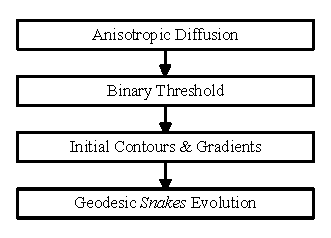
\includegraphics[width=3.2in]{Figures/gac/DataFlow.eps}
% \caption[主动脉内腔分割流程]{主动脉内腔分割流程。}
% \label{fig:aorta_data_flow}
\end{figure}
\end{frame}

\begin{frame}
\begin{itemize}
\item \textbf{原始图像的ROI提取}
\end{itemize}
\begin{figure}[t]
\centering
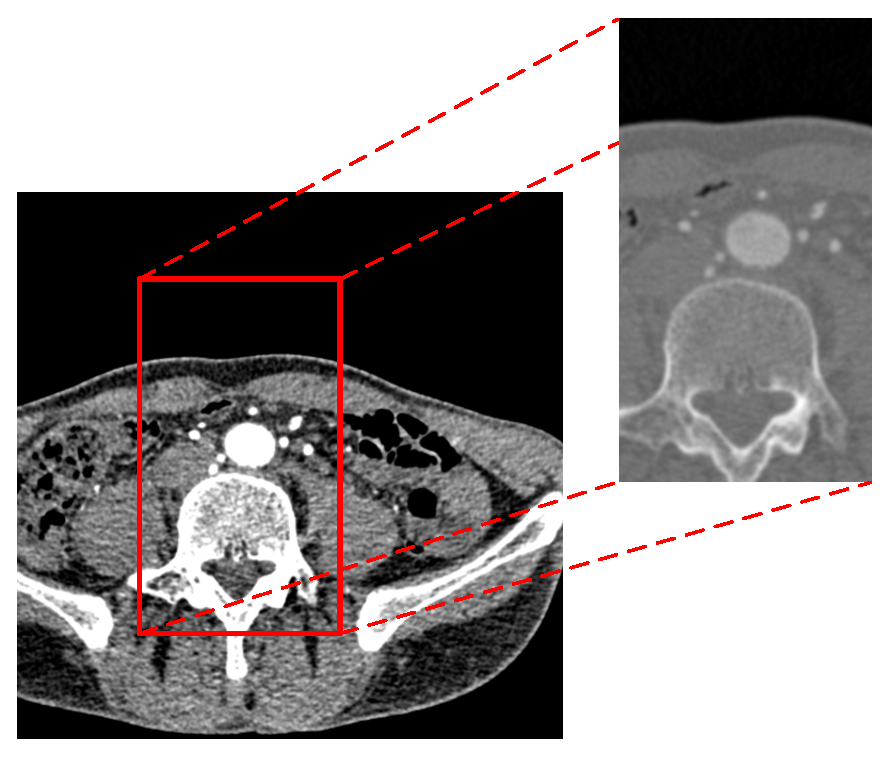
\includegraphics[width=2.0in]{../../Figures/gac/ROI.eps}
% \caption[原始图像的ROI提取]{原始图像的ROI提取。}
% \label{fig:aorta_roi}
\end{figure}
\end{frame}

\begin{frame}
\begin{itemize}
  \item \textbf{特征图像的生成步骤}:
  \begin{enumerate}
    \item 保护物体边缘的平滑处理($\text{传导参数} = 9.0$)
    \item 基于Gaussian核的梯度幅值计算($\sigma = 0.9$)
    \item 利用S型函数进行非线性映射($m = -3$, $n = 20$)
  \end{enumerate}
\end{itemize}
\begin{columns}[b,onlytextwidth]
\begin{column}{.3\textwidth}
\begin{figure}[t]
\centering
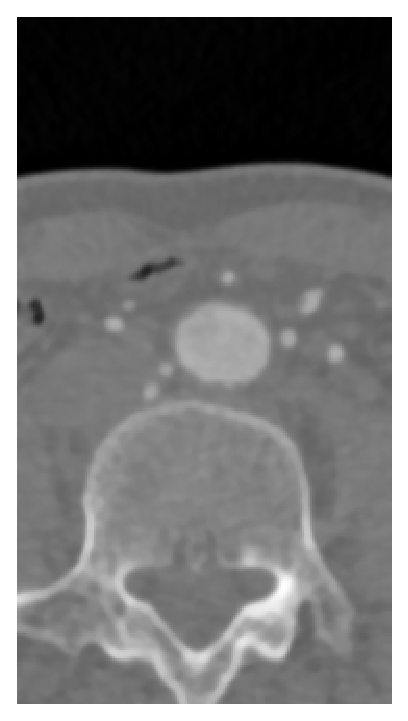
\includegraphics[height=1.5in]{../../Figures/gac/dcm_smoothing.eps}
\end{figure}
\end{column}
\begin{column}{.3\textwidth}
\begin{figure}[t]
\centering
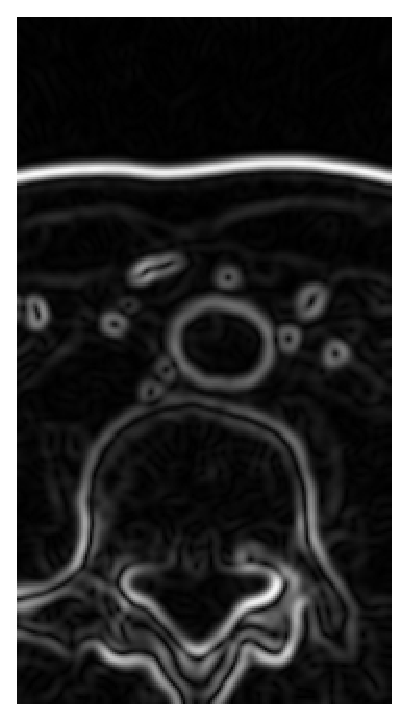
\includegraphics[height=1.5in]{../../Figures/gac/dcm_gradient.eps}
\end{figure}
\end{column}
\begin{column}{.3\textwidth}
\begin{figure}[t]
\centering
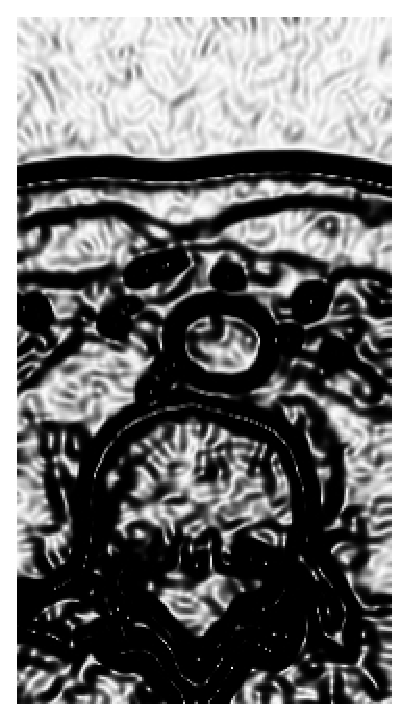
\includegraphics[height=1.5in]{../../Figures/gac/dcm_sigmoid.eps}
\end{figure}
\end{column}
\end{columns}
\end{frame}

\begin{frame}
\begin{itemize}
  \item \textbf{水平集演进过程}:
  \begin{enumerate}
    \item 阈值滤波($\text{TH}_{\text{lower}} = 300\text{HU}$, $\text{TH}_{\text{upper}} = 2000\text{HU}$)
    \item 从某一种子点开始,利用快速步进法进行的初始水平集演进
    \item 利用测地活动轮廓进行边缘检测(迭代次数: $100$)
    \item 利用二值阈值滤波完成像素亮度的反转(明亮区域的亮度值: $255$, 黑暗区域的亮度值: $0$)
  \end{enumerate}
\end{itemize}
\begin{columns}[b,onlytextwidth]
\begin{column}{.25\textwidth}
\begin{figure}[t]
\centering

\includegraphics[height=1.5in]{../../Figures/gac/dcm_threshold.eps}
\end{figure}
\end{column}
\begin{column}{.25\textwidth}
\begin{figure}[t]
\centering
\setlength{\fboxrule}{0.1pt}
\setlength{\fboxsep}{0cm}
\fbox{
\includegraphics[height=1.5in]{../../Figures/gac/dcm_fastMarching.eps}}
\end{figure}
\end{column}
\begin{column}{.25\textwidth}
\begin{figure}[t]
\centering
\setlength{\fboxrule}{0.1pt}
\setlength{\fboxsep}{0cm}
\fbox{
\includegraphics[height=1.5in]{../../Figures/gac/dcm_geodesic.eps}}
\end{figure}
\end{column}
\begin{column}{.25\textwidth}
\begin{figure}[t]
\centering
\includegraphics[height=1.5in]{../../Figures/gac/dcm_out.eps}
\end{figure}
\end{column}
\end{columns}
\end{frame} 

\begin{frame}
\begin{itemize}
  \item \textbf{主动脉内腔分割结果评估}:
  % \begin{enumerate}
    % \item 基于Jaccard系数
    % \item 基于Dice系数
  % \end{enumerate}
\end{itemize}
\begin{table}[t]
\renewcommand{\arraystretch}{0.5}
% \caption[主动脉内腔分割结果评估]{主动脉内腔表面模型分割结果评估}
% \label{tbl:aorta_evaluation}
\centering
\begin{tabular*}{75mm}{c c c}
\toprule
\hspace{2mm} \small{数据集序号}  & \hspace{2mm} \small{Jaccard}    & \hspace{2mm} \small{Dice}       \\
\midrule
\hspace{2mm} \small{1}           & \hspace{2mm} \small{$0.936434$} & \hspace{2mm} \small{$0.967174$} \\
\midrule
\hspace{2mm} \small{2}           & \hspace{2mm} \small{$0.928468$} & \hspace{2mm} \small{$0.962907$} \\
\midrule
\hspace{2mm} \small{3}           & \hspace{2mm} \small{$0.911307$} & \hspace{2mm} \small{$0.953595$} \\
\midrule
\hspace{2mm} \small{4}           & \hspace{2mm} \small{$0.918612$} & \hspace{2mm} \small{$0.957580$} \\
\midrule
\hspace{2mm} \small{5}           & \hspace{2mm} \small{$0.893099$} & \hspace{2mm} \small{$0.943531$} \\
\midrule
\hspace{2mm} \small{6}           & \hspace{2mm} \small{$0.953753$} & \hspace{2mm} \small{$0.976329$} \\
\midrule
\hspace{2mm} \small{7}           & \hspace{2mm} \small{$0.983812$} & \hspace{2mm} \small{$0.991840$} \\
\midrule
\hspace{2mm} \small{8}           & \hspace{2mm} \small{$0.922035$} & \hspace{2mm} \small{$0.959436$} \\
\midrule
\hspace{2mm} \small{9}           & \hspace{2mm} \small{$0.928791$} & \hspace{2mm} \small{$0.963081$} \\
\midrule
\hspace{2mm} \small{10}          & \hspace{2mm} \small{$0.937794$} & \hspace{2mm} \small{$0.967899$} \\
\midrule
\hspace{2mm} \small{11}          & \hspace{2mm} \small{$0.950207$} & \hspace{2mm} \small{$0.974468$} \\
\bottomrule
\end{tabular*}
\end{table}
\end{frame} 

\begin{frame}
\begin{itemize}
  \item \textbf{主动脉内腔分割结果评估}:
  \begin{enumerate}
    \item 基于Jaccard系数
    \item 基于Dice系数
  \end{enumerate}
\end{itemize}
\begin{columns}[b,onlytextwidth]
\begin{column}{.5\textwidth}
\begin{figure}[t]
\centering
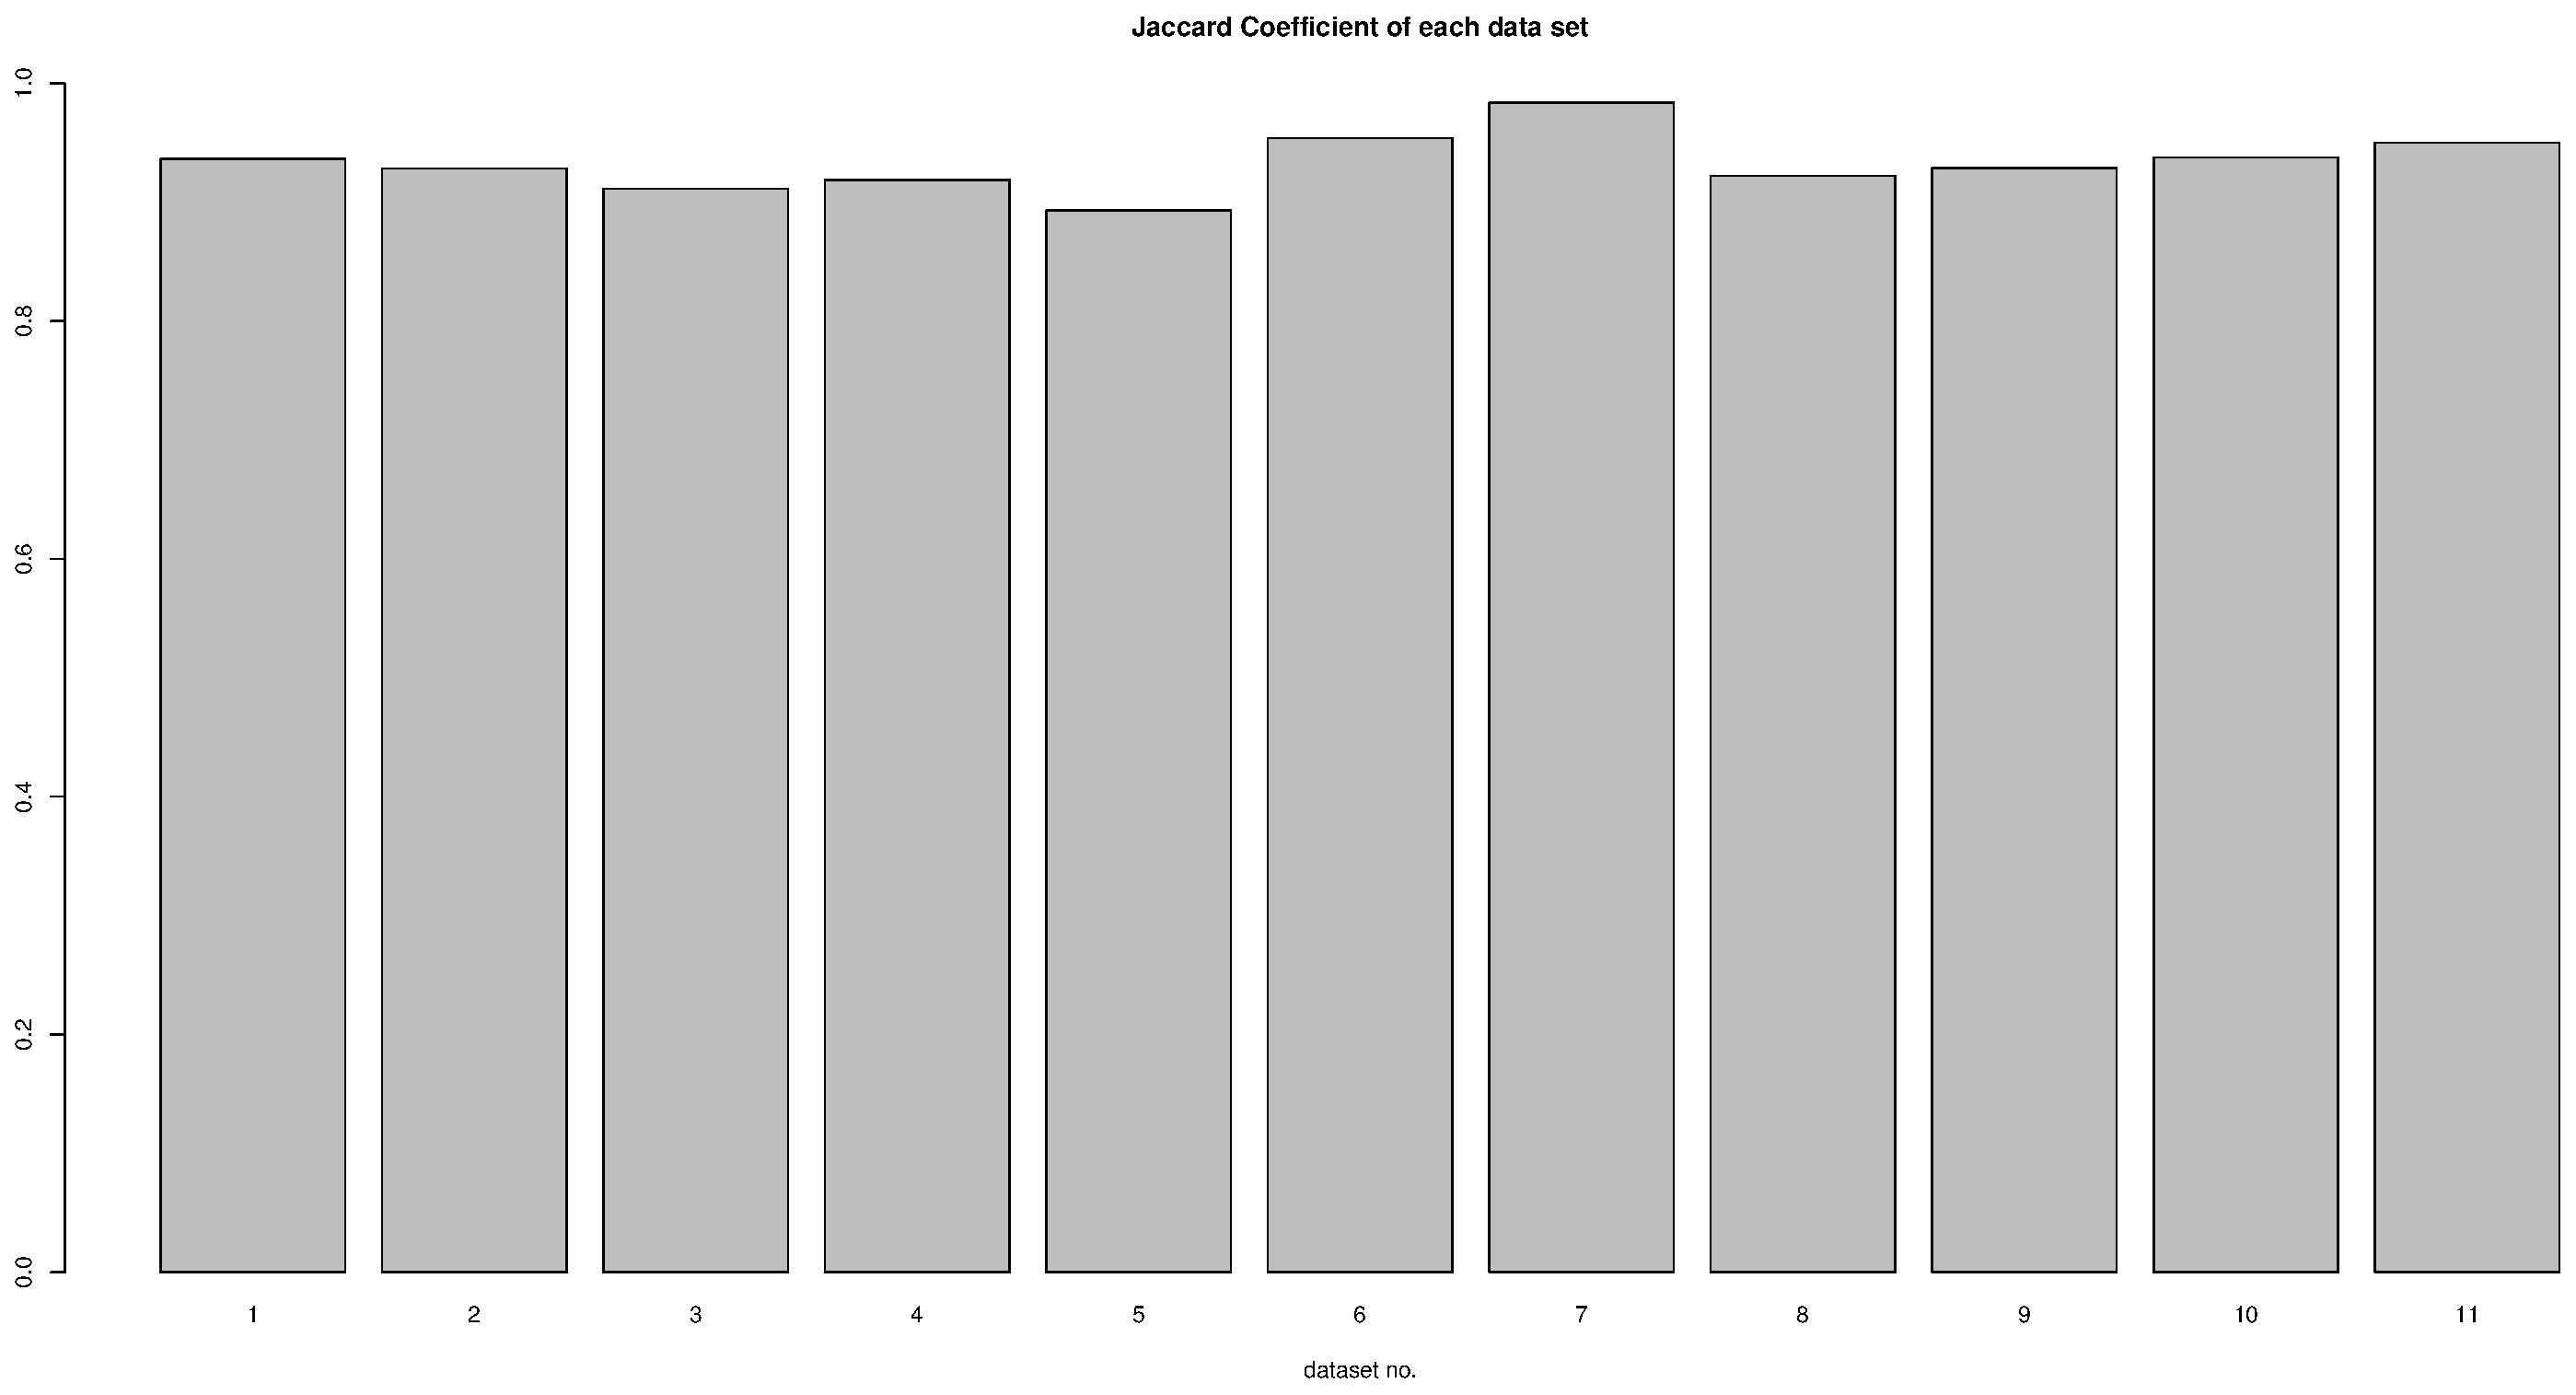
\includegraphics[width=1.5in,height=1.0in]{../../Figures/gac/Jaccard.eps}
\end{figure}
\end{column}
\begin{column}{.5\textwidth}
\begin{figure}[t]
\centering
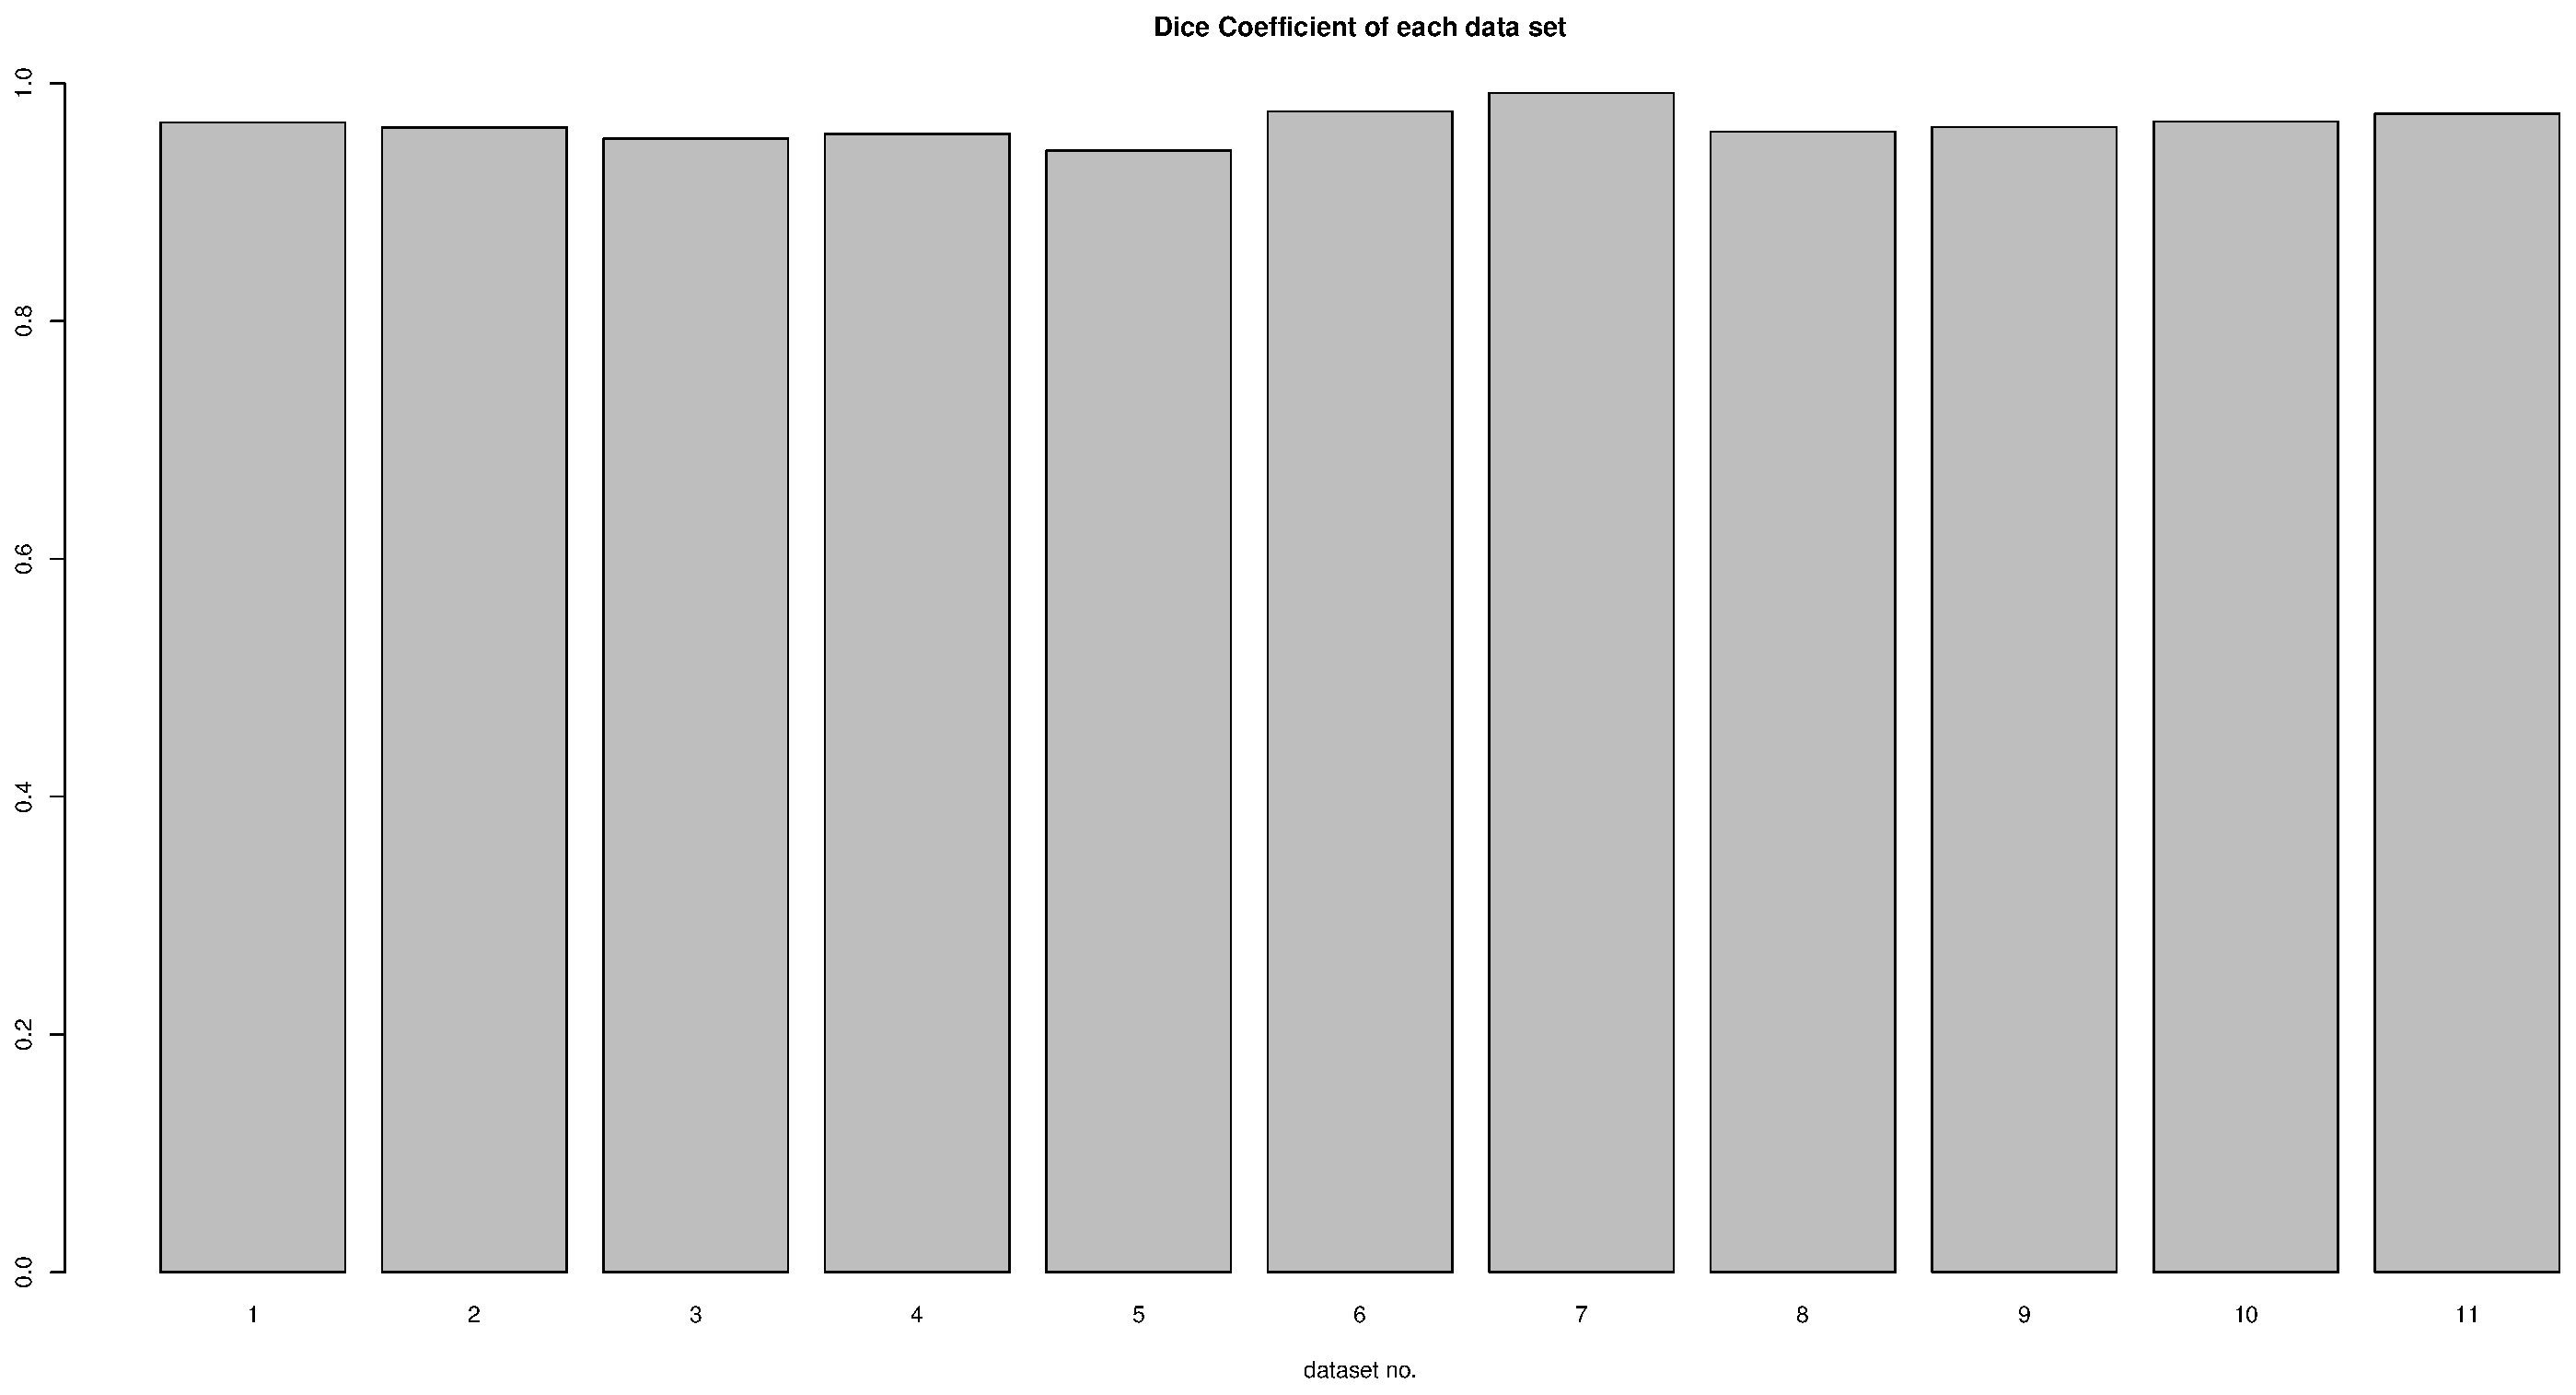
\includegraphics[width=1.5in,height=1.0in]{../../Figures/gac/Dice.eps}
\end{figure}
\end{column}
\end{columns}
\end{frame} 

\begin{frame}
\begin{itemize}
  \item \textbf{主动脉内腔三维模型}:
\end{itemize}
\begin{figure}[t]
\centering
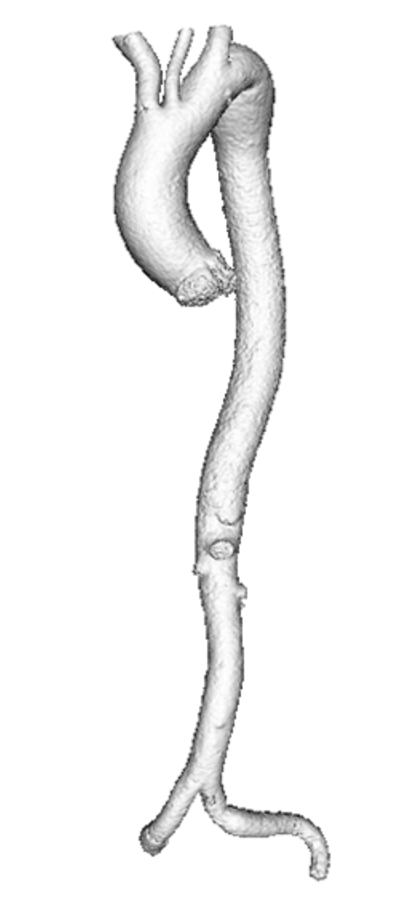
\includegraphics[height=1.8in]{../../Figures/gac/model.eps}
% \caption[主动脉内腔三维模型]{主动脉内腔三维模型。}
% \label{fig:aorta_visualization}
\end{figure} 
\end{frame} 

\begin{frame}

\end{frame} 